\section{Fundamento teórico}

Para comenzar se deben establecer unos parámetros para con la pala, ya que lo más básico de este trabajo empieza por determinar los efectos que produce la torsión en nuestra obtención de energía.

Es por ello que se determina que la pala de la turbina eólica es un trapecio cuya representación simplificada la vemos en la figura \ref{fig:pala_simp}

\begin{figure}[H]
    \centering
    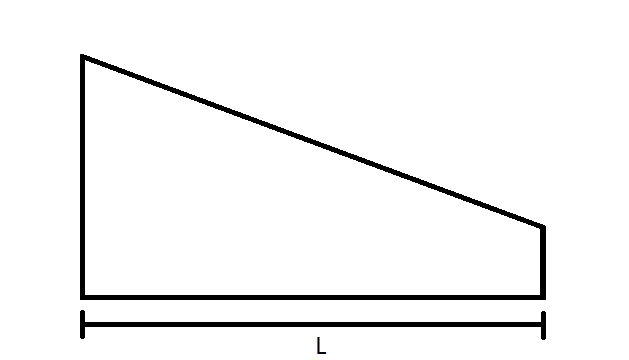
\includegraphics[width=0.7\textwidth]{images/pala turbina paint.png}
    \caption{Representación de una pala de turbina eólica}
    \label{fig:pala_simp}
\end{figure}


Lo siguiente que se debe hacer es dividir la pala de la figura \ref{fig:pala_simp} en un número de segmentos de igual largo, como se puede observar en la figura \ref{fig:pala_dividida}.
    \textbf{}
    \begin{figure}[H]
    \centering
    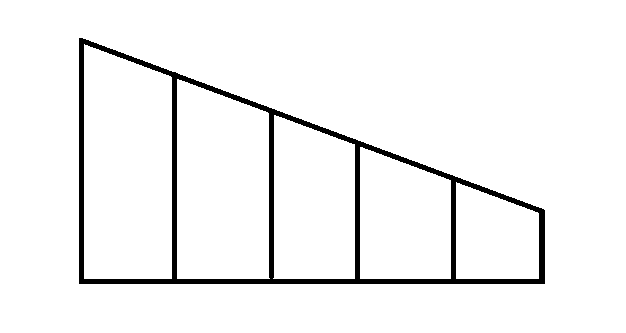
\includegraphics[width=0.7\textwidth]{images/pala dividida.png}
    \caption{Representación de una pala de turbina eólica en segmentos}
    \label{fig:pala_dividida}
\end{figure}

Por simplicidad, la pala se dividirá únicamente en $N$ segmentos, en este caso 5. Aunque se mantenga este valor durante el trabajo y es probable que no cambie, se asociará a una variable en caso de que se quieran hacer pruebas mediante MATLAB más adelante.
    
La longitud $L$ vista en la figura \ref{fig:pala_simp} es con la que se va a trabajar, por ello cada uno de los segmentos de la figura \ref{fig:pala_dividida} tendrá el siguiente largo $\dfrac{L}{N} = \dfrac{L}{5}$ ya que se dividió $N$ número de veces.


Como se puede observar en la figura \ref{fig:pala_dividida} cada segmento tiene una altura variable, esto se debe a la forma real de las palas, cuanto más cerca de la turbina mayor es el tamaño del segmento.\\\\

{\color{blue} La altura de estos segmentos depende del valor de una variable, conocida como longitud de cuerda, $c$, que varía dependiendo del segmento, cuanto más alejados del rotor menor será su valor.} \\\\

Se determina el área de los segmentos con la siguiente fórmula:

$$ area_{i} = \dfrac{L \cdot c_i}{N} $$
donde:
$$ i \in segmento $$
$$ segmento = \{1, ..., N\}$$

A continuación, se supone que los segmentos están separados los unos de los otros y ensartados por una línea imaginaria que ayudará al estudio de la torsión mediante giros de los segmentos alrededor suya.


\subsection{Estudio de los segmentos con giro inicial}

El ángulo $ \theta_1 $ se define como el giro inicial que sufrirán todos y cada uno de los segmentos que son paralelos al plano horizontal, desde el cual se presenta el viento que incidirá en nuestra pala.


El ángulo de torsión de cada segmento se define con la siguiente fórmula:

$$\theta_i =
\left\{\begin{matrix}
    \theta_1 \text{\hspace{77} si \hspace{1}} i=1 \\
    \sum_{k=1}^{i} \theta_k + \Delta_\theta \text{\hspace{20} si \hspace{2}} i>1 \\
    \end{matrix}$$